\documentclass[10pt, aspectratio=169, handout]{beamer}
\usefonttheme{professionalfonts}

\mode<presentation>
{
  \usetheme{Berkeley}
  \usecolortheme{beaver}
  \usefonttheme{default}
  \setbeamertemplate{navigation symbols}{}
  \setbeamertemplate{caption}[numbered]
} 

\setbeamertemplate{footline}{%
  \leavevmode%
  \hbox{%
    \begin{beamercolorbox}[wd=.85\paperwidth,ht=2.5ex,dp=1ex,left]{author in head/foot}%
      \usebeamerfont{author in head/foot}Maxx Seminario, Electronic Circuits, Spring 2026%
    \end{beamercolorbox}%
    \begin{beamercolorbox}[wd=.15\paperwidth,ht=2.5ex,dp=1ex,right]{date in head/foot}%
      \hspace*{0.5em}\insertframenumber{} / \inserttotalframenumber\hspace*{0.5em}%
    \end{beamercolorbox}%
  }%
  \vskip0pt%
}

\usepackage[english]{babel}
\usepackage[utf8]{inputenc}
\usepackage{tikz}
\usepackage{pgfplots}
\usepackage{array}
\usepackage{makecell}
\usepackage{verbatim}
\usepackage{graphicx}
\usepackage{subcaption}
\usepackage{amsfonts}
\usepackage{amsmath}
\usepackage{bm}
\usepackage{epstopdf}
\usepackage[american]{circuitikz}
\usepackage{caption}
\captionsetup{compatibility=false}
\usepackage[absolute,overlay]{textpos}
\usetikzlibrary{calc}
\usetikzlibrary{pgfplots.fillbetween, backgrounds}
\usetikzlibrary{positioning}
\usetikzlibrary{pgfplots.groupplots}
\usetikzlibrary{plotmarks}
\usetikzlibrary{calc}
\usetikzlibrary{decorations.markings}
\usetikzlibrary{arrows.meta,calc}

\usepgfplotslibrary{groupplots}
\pgfplotsset{compat=newest} 

\usepackage{hyperref}
\hypersetup{
    colorlinks=true,
    linkcolor=blue,
    filecolor=magenta,      
    urlcolor=cyan,
}

% Added by Maxx Seminario 01/06/2026 - for colored icons in itemize labels
\usepackage{wasysym} % for smiles and frowns
\newcommand{\neutralface}{%
  \tikz[baseline=-0.6ex]{
    \draw (0,0) circle (0.9ex);
    \fill (-0.35ex,0.25ex) circle (0.12ex);
    \fill ( 0.35ex,0.25ex) circle (0.12ex);
    \draw (-0.35ex,-0.25ex) -- (0.35ex,-0.25ex);
  }%
}
\newcommand{\baditem}{\textcolor{red!70!black}{\frownie}}
\newcommand{\gooditem}{\textcolor{green!60!black}{\smiley}}
\newcommand{\mehitem}{\textcolor{orange!80!black}{\neutralface}}

\title[ECEN 222]{Diode Applications: Rectifiers and Power Supplies}
\author{Maxx Seminario}
\institute{University of Nebraska-Lincoln}
\date{Spring 2026}

\begin{document}
\begin{frame}
  \titlepage
\end{frame}

\section{Introduction}

\begin{frame}{Diode Applications Overview}
    
    \begin{columns}[t]
    \column{0.48\textwidth}
        \textbf{Why Study Rectifiers?}:
        \begin{itemize}
            \item Most electronics need DC power
            \item Wall outlets provide AC power
            \item Rectifiers convert AC to DC
            \item Foundation of power supplies
        \end{itemize}
        
        \vspace{0.5em}
        \textbf{Key Applications}:
        \begin{itemize}
            \item Battery chargers
            \item Computer power supplies
            \item LED drivers
            \item Motor controllers
        \end{itemize}
    
    \column{0.48\textwidth}
        \textbf{Topics We'll Cover}:
        \begin{itemize}
            \item Half-wave rectifiers
            \item Full-wave rectifiers
            \item Bridge rectifiers
            \item Filtering capacitors
            \item Ripple voltage
            \item Voltage regulation with Zeners
        \end{itemize}
        
        \vspace{0.5em}
        \begin{center}
        \begin{circuitikz}[scale=0.8]
            \draw (0,0) to[sV, l=$v_{AC}$] (0,2)
                to[D] (2,2)
                to[R, l=$R_L$] (2,0)
                to[short] (0,0);
            \draw (3,1) node[right] {Simple Rectifier};
        \end{circuitikz}
        \end{center}
    
    \end{columns}
    
\end{frame}

\section{Half-Wave Rectifiers}

\begin{frame}{Half-Wave Rectifier Circuit}
    
    \begin{columns}[t]
    \column{0.48\textwidth}
        \textbf{Basic Circuit}:
        
        \begin{center}
        \begin{circuitikz}[american, scale=0.8]
            \draw (0,0) to[sV, l=$v_{AC}$] (0,3)
                  to[D, l=$D$] (3,3)
                  to[R, l=$R_L$, v=$v_o$] (3,0)
                  to[short] (0,0);
            \draw (1.5,0) node[ground]{};
        \end{circuitikz}
        \end{center}
        
        \vspace{-0.5cm}

        \textbf{Operation}:
        \begin{itemize}
            \item Input: $v_{AC} = V_p \sin(\omega t)$
            \item Positive half-cycle: diode ON
            \item Negative half-cycle: diode OFF
            \item Output: positive half-waves only
        \end{itemize}
        
    \column{0.48\textwidth}
        \textbf{Waveforms}:
        
        \begin{center}
        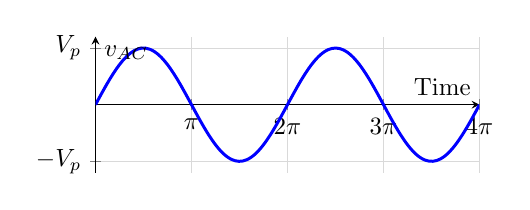
\begin{tikzpicture}[scale=0.9]
            \begin{axis}[
                width=7cm, 
                height=3.5cm,
                xlabel={Time},
                ylabel={$v_{AC}$},
                xmin=0, 
                xmax=4*pi,
                ymin=-1.2, 
                ymax=1.2,
                grid=major,
                grid style={line width=0.1pt, draw=gray!30},
                axis lines=middle,
                xtick={0, pi, 2*pi, 3*pi, 4*pi},
                xticklabels={0, $\pi$, $2\pi$, $3\pi$, $4\pi$},
                ytick={-1,0,1},
                yticklabels={$-V_p$,0,$V_p$},
            ]
            \addplot[blue, very thick, smooth, domain=0:4*pi, samples=100] {sin(deg(x))};
            \end{axis}
        \end{tikzpicture}
        
        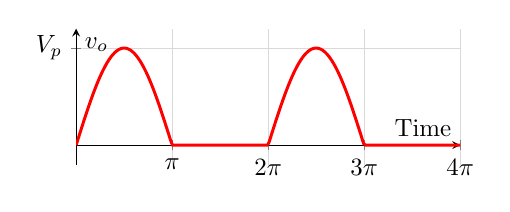
\begin{tikzpicture}[scale=0.9]
            \begin{axis}[
                width=7cm, 
                height=3.5cm,
                xlabel={Time},
                ylabel={$v_o$},
                xmin=0, 
                xmax=4*pi,
                ymin=-0.2, 
                ymax=1.2,
                grid=major,
                grid style={line width=0.1pt, draw=gray!30},
                axis lines=middle,
                xtick={0, pi, 2*pi, 3*pi, 4*pi},
                xticklabels={0, $\pi$, $2\pi$, $3\pi$, $4\pi$},
                ytick={0,1},
                yticklabels={0,$V_p$},
            ]
            \addplot[red, very thick, smooth, domain=0:4*pi, samples=200] {max(sin(deg(x)),0)};
            \end{axis}
        \end{tikzpicture}
        \end{center}
        
    \end{columns}
    
\end{frame}

\begin{frame}{Half-Wave Rectifier Analysis}
    
    \begin{columns}[t]
    \column{0.48\textwidth}
        \textbf{Average (DC) Output Voltage}:
        
        For ideal diode ($V_D = 0$):
        \begin{equation*}
            V_{DC} = \frac{V_p}{\pi} \approx 0.318 V_p
        \end{equation*}
        
        For real silicon diode ($V_D \approx 0.7$ V):
        \begin{equation*}
            V_{DC} = \frac{V_p - V_D}{\pi}
        \end{equation*}
        
        \vspace{0.5em}
        \textbf{Peak Inverse Voltage (PIV)}:
        \begin{itemize}
            \item Maximum reverse voltage on diode
            \item Must select diode with PIV $> V_p$
            \item Else, diode may break down during negative half-cycle
        \end{itemize}
        
    \column{0.48\textwidth}
        \textbf{Example Calculation}:
        
        Given: $V_{AC,RMS} = 12$ V
        
        \begin{enumerate}
            \item Peak voltage: \\
            $V_p = \sqrt{2} \times V_{RMS} = 17$ V
            
            \item Calculate DC output: \\
            $V_{DC} = \frac{17 - 0.7}{\pi} = \frac{16.27}{\pi} = 5.18$ V
            
            \item PIV requirement: \\
            PIV $\geq 17$ V
        \end{enumerate}
        
        \vspace{0.5em}
        \textbf{Limitations}:
        \begin{itemize}
            \item[\baditem] Low DC output (only 31.8\%)
            \item[\baditem] Poor power utilization
            \item[\baditem] Large ripple voltage
        \end{itemize}
        
    \end{columns}
    
\end{frame}

\begin{frame}{Half-Wave Rectifier with Filter Capacitor}
    
    \begin{columns}[t]
    \column{0.48\textwidth}
        \textbf{Filtered Rectifier}:
        
        \begin{center}
        \begin{circuitikz}[american, scale=0.8]
            \draw (0,0) to[sV, l=$v_{AC}$] (0,3)
                  to[D, l=$D$] (3,3)
                  to[short] (4.5,3);
            \draw (3,3) to[R, l=$R_L$, v=$v_o$] (3,0);
            \draw (4.5,3) to[C, l=$C$] (4.5,0);
            \draw (0,0) to[short] (4.5,0);
            \draw (2.25,0) node[ground]{};
        \end{circuitikz}
        \end{center}
        
        \vspace{-0.5cm}

        \textbf{Operation}:
        \begin{itemize}
            \item Capacitor charges to $\approx V_p$ 
            \item Capacitor discharges through $R_L$ 
            \item Creates "ripple" voltage
            \item DC voltage higher than unfiltered
        \end{itemize}
        
    \column{0.48\textwidth}
        \textbf{Output Waveform}:
        
        \begin{center}
        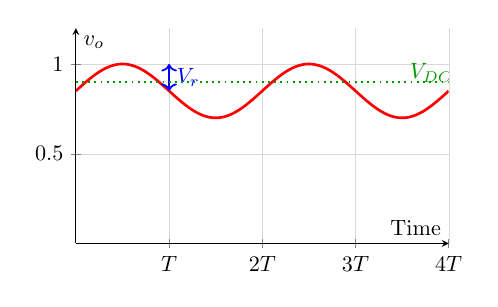
\begin{tikzpicture}[scale=0.8]
            \begin{axis}[
                width=7.5cm, 
                height=5cm,
                xlabel={Time},
                ylabel={$v_o$},
                xmin=0, 
                xmax=4*pi,
                ymin=0, 
                ymax=1.2,
                grid=major,
                grid style={line width=0.1pt, draw=gray!30},
                axis lines=middle,
                xtick={0, pi, 2*pi, 3*pi, 4*pi},
                xticklabels={0, $T$, $2T$, $3T$, $4T$},
            ]
            
            % Draw envelope
            \addplot[red, very thick, domain=0:4*pi, samples=200] 
                {max(0.85 + 0.15*sin(deg(x)), sin(deg(x)))};
            
            % Annotate ripple
            \draw[<->, blue, thick] (axis cs:pi,0.85) -- (axis cs:pi,1.0);
            \node[blue, right] at (axis cs:pi,0.925) {$V_r$};
            
            % Draw DC level line
            \draw[green!60!black, thick, dotted] (axis cs:0,0.9) -- (axis cs:4*pi,0.9);
            \node[green!60!black, right] at (axis cs:3.5*pi,0.95) {$V_{DC}$};
            
            \end{axis}
        \end{tikzpicture}
        \end{center}
        
        \vspace{-0.3cm}
        \textbf{Ripple Voltage}:
        \begin{equation*}
            V_r \approx \frac{V_p}{f R_L C}
        \end{equation*}
        
    \end{columns}
    
\end{frame}

\begin{frame}{Ripple Voltage Analysis}
    
    \begin{columns}[t]
    \column{0.48\textwidth}
        \textbf{Key Equations}:
        
        Ripple voltage (peak-to-peak):
        \begin{equation*}
            V_r \approx \frac{V_p}{f R_L C}
        \end{equation*}

        \vspace{-0.4cm}
        
        DC output voltage:
        \begin{equation*}
            V_{DC} \approx V_p - \frac{V_r}{2}
        \end{equation*}

        \vspace{-0.5cm}
        
        Ripple factor:
        \begin{equation*}
            r = \frac{V_{r,RMS}}{V_{DC}}
        \end{equation*}

        \vspace{-0.3cm}

        \textbf{Design Guidelines}:
        \begin{itemize}
            \item[\gooditem] Larger $C$ reduces ripple
            \item[\gooditem] Larger $R_L$ reduces ripple
            \item[\gooditem] Higher frequency reduces ripple
        \end{itemize}
        
    \column{0.48\textwidth}
        \textbf{Example}:
        
        Given: 
        \begin{itemize}
            \item $V_p = 17$ V
            \item $f = 60$ Hz
            \item $R_L = 2.2$ k$\Omega$
            \item $C = 470$ $\mu$F
        \end{itemize}
        
        Calculate ripple:
        \begin{align*}
            V_r &= \frac{17}{60 \times 2200 \times 470 \times 10^{-6}} = 0.274 \text{ V}
        \end{align*}

        \vspace{-0.2cm}

        \begin{equation*}
            V_{DC} = 17 - \frac{0.274}{2} = 16.86 \text{ V}
        \end{equation*}
        
        \vspace{-0.3cm}
        \textbf{Trade-offs}:
        \begin{itemize}
            \item Large $C$: less ripple, larger size
            \item Peak diode current increases with $C$
        \end{itemize}
        
    \end{columns}
    
\end{frame}

\section{Full-Wave Rectifiers}

\begin{frame}{Bridge Rectifier Circuit}
    
    \begin{columns}[t]
    \column{0.48\textwidth}
        \textbf{Bridge Configuration}:
        
        \begin{center}
        \begin{circuitikz}[american, scale=.55]
            % \draw[step=1cm, gray!30, very thin] (-2,-2) grid (8,6);
            \ctikzset{label/align=straight}
            \draw (-1,0) to[sV, l=$v_{AC}$] (-1,4);
            \draw (-1,4) -- (4,4);
            \ctikzset{label distance=-.2cm}
            \draw (2,2) to [D, l=$D_4$, *-*] (4,4) to [D, l=$D_1$, *-*] (6,2);
            \draw (2,2) to [D, l_=$D_2$, *-*] (4,0) to [D, l_=$D_3$, *-*] (6,2);
            \draw (-1,0) -- (4,0);
            \ctikzset{label distance=0}
            \draw (6,2) -- (8,2) to [R, l^=$R_L$, v_=$v_o$] (8,-1) to node[ground]{} (1, -1) -- (1,2) -- (2,2);
            % \draw (8,2) -- (10,2) to [cC, l^=$C$] (10,-1) -- (8,-1);

        \end{circuitikz}
        \end{center}
        
        \vspace{-0.8cm}
        \textbf{Operation}:
        \begin{itemize}
            \item Positive half-cycle: $D_1$, $D_2$ conduct
            \item Negative half-cycle: $D_3$, $D_4$ conduct
            \item Both half-cycles produce output
            \item Two diodes always in series
        \end{itemize}
        
    \column{0.48\textwidth}
        \textbf{Output Characteristics}:
        \begin{itemize}
            \item $v_o$ is always positive
            \item Output is full-wave rectified
            \item Continuous current through load
        \end{itemize}
        
        \vspace{0.5em}
        \textbf{Advantages}:
        \begin{itemize}
            \item[\gooditem] No center-tap transformer needed
            \item[\gooditem] Full-wave rectification
            \item[\gooditem] Higher DC output
            \item[\gooditem] Lower ripple frequency (2$f$)
        \end{itemize}
        
        \textbf{Disadvantages}:
        \begin{itemize}
            \item[\baditem] Two diode drops ($\approx 1.4$ V)
            \item[\baditem] Requires four diodes
        \end{itemize}
        
    \end{columns}

\end{frame}

\begin{frame}{Bridge Rectifier Analysis}
    
    \begin{columns}[t]
    \column{0.48\textwidth}
        \textbf{DC Output Voltage}:
        
        For ideal diodes ($V_D = 0$):
        \begin{equation*}
            V_{DC} = \frac{2V_p}{\pi} \approx 0.637 V_p
        \end{equation*}
        
        For real silicon diodes ($V_D \approx 0.7$ V each):
        \begin{equation*}
            V_{DC} = \frac{2(V_p - 2V_D)}{\pi}
        \end{equation*}
        
        \textbf{Comparison to Half-Wave}:
        \begin{itemize}
            \item DC output is 2x higher
            \item Ripple frequency is 2x higher
            \item Better power utilization
        \end{itemize}
        
    \column{0.48\textwidth}
        \textbf{Output Waveform}:
        
        \begin{center}
        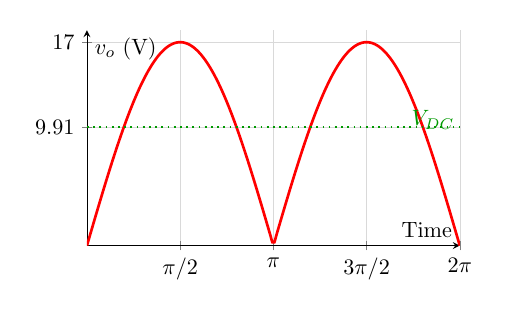
\begin{tikzpicture}[scale=0.8]
            \begin{axis}[
                width=7.5cm, 
                height=5cm,
                xlabel={Time},
                ylabel={$v_o$ (V)},
                xmin=0, 
                xmax=2*pi,
                ymin=0, 
                ymax=18,
                grid=major,
                grid style={line width=0.1pt, draw=gray!30},
                axis lines=middle,
                xtick={0, pi/2, pi, 3*pi/2, 2*pi},
                xticklabels={0, $\pi/2$, $\pi$, $3\pi/2$, $2\pi$},
                ytick={0, 9.91, 17},
                yticklabels={0, 9.91, 17},
            ]
            \addplot[red, very thick, smooth, domain=0:2*pi, samples=200] {17*abs(sin(deg(x)))};
            
            % Draw DC level line
            \draw[green!60!black, thick, dotted] (axis cs:0,9.91) -- (axis cs:2*pi,9.91);
            \node[green!60!black, right] at (axis cs:1.7*pi,10.5) {$V_{DC}$};
            \end{axis}
        \end{tikzpicture}
        \end{center}
        
        \vspace{-0.75cm}
        \textbf{Example}:
        
        $V_{AC,RMS} = 12$ V, $V_p = 17$ V
        
        \begin{equation*}
            V_{DC} = \frac{2(17 - 1.4)}{\pi} = \frac{31.14}{\pi} = 9.91 \text{ V}
        \end{equation*}

        \vspace{-0.1cm}
        
        Compare to half-wave: 5.18 V (nearly 2x improvement)
        
    \end{columns}
    
\end{frame}

\begin{frame}{Bridge Rectifier with Filter}
    
    \begin{columns}[T]
    \column{0.6\textwidth}
        \textbf{Filtered Bridge Rectifier}:

        \vspace{-0.4cm}
        
        \begin{center}
        \begin{circuitikz}[american, scale=.55]
                % \draw[step=1cm, gray!30, very thin] (-2,-2) grid (8,6);
                \ctikzset{label/align=straight}
                \draw (-1,0) to[sV, l=$v_{AC}$] (-1,4);
                \draw (-1,4) -- (4,4);
                \ctikzset{label distance=-.2cm}
                \draw (2,2) to [D, l=$D_4$, *-*] (4,4) to [D, l=$D_1$, *-*] (6,2);
                \draw (2,2) to [D, l_=$D_2$, *-*] (4,0) to [D, l_=$D_3$, *-*] (6,2);
                \draw (-1,0) -- (4,0);
                \ctikzset{label distance=0}
                \draw (6,2) -- (8,2) to [R, l^=$R_L$, v_=$v_o$] (8,-1) to node[ground]{} (1, -1) -- (1,2) -- (2,2);
                \draw (8,2) -- (10,2) to [cC, l^=$C$] (10,-1) -- (8,-1);

            \end{circuitikz}
        \end{center}
        
        \vspace{0.5em}
        \textbf{Key Difference}:
        
        Ripple frequency is \textbf{2$f$} 

        \vspace{-0.2cm}
        
        \begin{equation*}
            V_r \approx \frac{V_p}{2f R_L C}
        \end{equation*}

        \vspace{-0.1cm}
        
        Ripple is \textbf{half} that of half-wave rectifier with same $C$!
        
    \column{0.4\textwidth}
        % \textbf{Output Waveform}:
        
        \begin{center}
        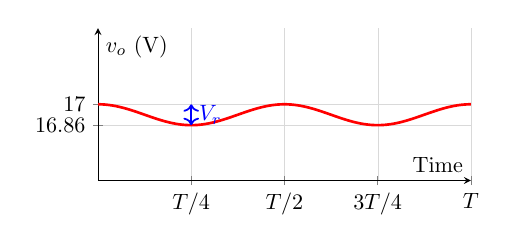
\begin{tikzpicture}[scale=0.8]
            \begin{axis}[
                width=7.5cm, 
                height=4cm,
                xlabel={Time},
                ylabel={$v_o$ (V)},
                xmin=0, 
                xmax=2*pi,
                ymin=16.5, 
                ymax=17.5,
                grid=major,
                grid style={line width=0.1pt, draw=gray!30},
                axis lines=middle,
                xtick={0, pi/2, pi, 3*pi/2, 2*pi},
                xticklabels={0, $T/4$, $T/2$, $3T/4$, $T$},
                ytick={16.5, 16.863, 17},
                yticklabels={16.5, 16.86, 17},
            ]
            
            % Approximation of filtered output
            \addplot[red, very thick, domain=0:2*pi, samples=400] 
                {16.9315 + 0.0685*cos(2*deg(x))};
            
            \draw[<->, blue, thick] (axis cs:pi/2,16.863) -- (axis cs:pi/2,17);
            \node[blue, right] at (axis cs:pi/2,16.93) {$V_r$};
            
            \end{axis}
        \end{tikzpicture}
        \end{center}
        
        \vspace{-0.3cm}
        \textbf{Design Example}:
        
        Same as before, but $f$ → $2f$:

        \vspace{-0.5cm}
        
        \begin{align*}
            V_r &= \frac{17}{2 \times 60 \times 2200 \times 470 \mu} = 0.137 \text{ V}
        \end{align*}

        \vspace{-0.2cm}

        \begin{equation*}
            V_{DC} = 17 - \frac{0.137}{2} = 16.93 \text{ V}
        \end{equation*}
        
    \end{columns}
    
\end{frame}

\section{Voltage Regulation}

\begin{frame}{Need for Voltage Regulation}
    \begin{columns}[t]
    \column{0.48\textwidth}
        \textbf{The Problem}:
        
        \begin{itemize}
            \item Rectifier output varies with:
            \begin{itemize}
                \item Input voltage changes
                \item Load current changes
                \item Ripple voltage
            \end{itemize}
            \item Most circuits need stable DC
            \item Example: Logic circuits need ±5\% tolerance
        \end{itemize}
        
        
    \column{0.48\textwidth}
        \textbf{The Solution}:
        
        Voltage regulator:
        \begin{itemize}
            \item Maintains constant output voltage
            \item Compensates for input variations
            \item Compensates for load variations
            \item Types: Linear, switching, Zener
        \end{itemize}
        
        \vspace{0.5em}
        \textbf{Performance Metrics}:
        \begin{itemize}
            \item \textbf{Load regulation}: how much $V_o$ changes with load
            \item \textbf{Line regulation}: how much $V_o$ changes with input
            \item \textbf{Efficiency}: $P_{out}/P_{in}$
        \end{itemize}
        
    \end{columns}
    
\end{frame}

\begin{frame}{Zener Diode Shunt Regulator}
    
    \begin{columns}[t]
    \column{0.48\textwidth}
        \textbf{Basic Shunt Regulator}:
        \vspace{-0.5cm}
        \begin{center}
        \begin{circuitikz}[american, scale=0.9]
            \draw (0,3) to[V, l=$V_{in}$] (0,0);
            \draw (0,3) to[R, l=$R_S$, i>^=$I_S$] (3,3);
            
            % Zener branch 
            \draw (3,3) to[short] (4.0,3)
                  to[zD, l_=$D_Z$, v^=$V_Z$, i>_=$I_Z$, invert] (4.0,0);
            
            % Load branch 
            \draw (3,3) to[short] (6,3)
                  to[R, l_=$R_L$, v^=$V_o$, i>_=$I_L$] (6,0);
            
            % Return
            \draw (0,0) to[short] (6,0);
            \draw (3,0) node[ground]{};
        \end{circuitikz}
        \end{center}
        
        \vspace{-0.4cm}
        \textbf{Operation Principle}:
        \begin{itemize}
            \item Zener maintains constant $V_Z$
            \item $R_S$ drops excess voltage
            \item Zener absorbs current variations
            \item $I_S = I_Z + I_L$ (KCL)
        \end{itemize}
        
    \column{0.48\textwidth}
        \textbf{Equations of Note}:
        
        Series resistor current:
        \begin{equation*}
            I_S = \frac{V_{in} - V_Z}{R_S}
        \end{equation*}

        \vspace{-0.3cm}
        
        Kirchhoff's current law:
        \begin{equation*}
            I_Z = I_S - I_L
        \end{equation*}

        \vspace{-0.3cm}
        
        Zener power dissipation:
        \begin{equation*}
            P_Z = V_Z \cdot I_Z
        \end{equation*}
        
        \vspace{-0.3cm}
        \textbf{Design Constraints}:
        \begin{itemize}
            \item $I_Z \geq I_{Z,min}$ (stay in breakdown)
            \item $P_Z \leq P_{Z,max}$ (power rating)
            \item Worst case: max $I_L$, min $V_{in}$
            \item Best efficiency at full load
        \end{itemize}
        
    \end{columns}
    
\end{frame}

\begin{frame}{Shunt Regulator Design Example}
    
    \begin{columns}[t]
    \column{0.48\textwidth}
        \textbf{Design Specifications}:
        
        \begin{itemize}
            \item Output: $V_o = 5.1$ V (use 5.1 V Zener)
            \item Input: $V_{in} = 12$ V (from rectifier)
            \item Load: $I_L = 0$ to 50 mA
            \item Zener: $I_{Z,min} = 5$ mA, $P_{Z,max} = 0.5$ W
        \end{itemize}
        
        \textbf{Design Process}:
        
        \textbf{Step 1}: Find maximum safe $I_Z$ 

        \vspace{-0.25cm}
        
        \begin{equation*}
            I_{Z,max} = \frac{P_{Z,max}}{V_Z} = \frac{0.5}{5.1} = 98 \text{ mA}
        \end{equation*}
        
        \textbf{Step 2}: Choose $I_S$ for no-load condition:
        
        At no load, $I_Z = I_S$, so choose $I_S = 90$ mA (safe margin below 98 mA)
        
    \column{0.48\textwidth}
        \textbf{Step 3}: Calculate $R_S$

        \vspace{-0.25cm}
        
        \begin{equation*}
            R_S = \frac{V_{in} - V_Z}{I_S} = \frac{12 - 5.1}{0.09} = 76.7 \text{ }\Omega
        \end{equation*}
        
        \vspace{0.5em}
        \textbf{Step 4}: Verify operation at both extremes
        
        At no load ($I_L = 0$):
        \begin{align*}
            I_Z &= I_S = 90 \text{ mA} \\
            P_Z &= 5.1 \times 0.09 = 459 \text{ mW} 
        \end{align*}
        
        At full load ($I_L = 50$ mA):
        \begin{align*}
            I_Z &= 90 - 50 = 40 \text{ mA} \\
            &> I_{Z,min} = 5 \text{ mA} 
        \end{align*} 
        
    \end{columns}
    
\end{frame}

\begin{frame}{Regulation Performance}
    
    \begin{columns}[t]
    \column{0.48\textwidth}
        \textbf{Load Regulation}:
        
        Measures output voltage change with load current:
        
        \begin{equation*}
            \text{Load Reg} = \frac{V_{o,no-load} - V_{o,full-load}}{V_{o,full-load}} \times 100\%
        \end{equation*}
  
        Affected by:
        \begin{itemize}
            \item Zener dynamic resistance $r_z$
            \item Series resistance $R_S$
            \item Load current range
        \end{itemize}

    \column{0.48\textwidth}
        \textbf{Line Regulation}:
        
        Measures output voltage change with input voltage:

        \vspace{-0.1cm}
        
        \begin{equation*}
            \text{Line Reg} = \frac{\Delta V_o}{\Delta V_{in}} \times 100\%
        \end{equation*}

        \vspace{-0.1cm}

        \textbf{Efficiency}:
        
        \begin{equation*}
            \eta = \frac{P_o}{P_{in}} = \frac{V_o I_L}{V_{in} I_S} \times 100\%
        \end{equation*}
        
        
        \vspace{-0.1cm}
        \textbf{Key Points}:
        \begin{itemize}
            \item[\baditem] Shunt regulators have poor efficiency
            \item[\baditem] Power wasted in $R_S$ and Zener
            \item[\gooditem] Simple and inexpensive
            \item[\gooditem] Good for low-power applications
        \end{itemize}
        
    \end{columns}
    
\end{frame}

\section{Summary}

\begin{frame}{Summary: Diode Applications}
    
    \begin{columns}[t]
    \column{0.48\textwidth}
        \textbf{Rectifier Circuits}:
        
        Half-Wave:
        \begin{itemize}
            \item $V_{DC} = V_p/\pi \approx 0.318 V_p$
            \item Ripple frequency $= f$
            \item Low efficiency
        \end{itemize}
        
        Bridge (Full-Wave):
        \begin{itemize}
            \item $V_{DC} = 2V_p/\pi \approx 0.637 V_p$
            \item Ripple frequency $= 2f$
            \item Better efficiency
        \end{itemize}
        
        \vspace{-0.1cm}
        \textbf{Filtering}:
        \begin{itemize}
            \item Capacitor smooths output
            \item $V_r \approx V_p/(f R_L C)$
            \item Larger $C$ reduces ripple
        \end{itemize}
        
    \column{0.48\textwidth}
        \textbf{Voltage Regulation}:
        
        Zener Shunt Regulator:
        \begin{itemize}
            \item Maintains constant output
            \item $I_S = I_Z + I_L$
            \item $R_S = (V_{in} - V_Z)/I_S$
            \item Check power dissipation
        \end{itemize}
        
        Performance:
        \begin{itemize}
            \item Load regulation: $\Delta V_o$ with $\Delta I_L$
            \item Line regulation: $\Delta V_o$ with $\Delta V_{in}$
            \item Efficiency: typically 20-50\%
        \end{itemize}
        
        
    \end{columns}

    
\end{frame}

\end{document}
